\section{End-to-End Network Training}

\emph{End-to-end network training} is a deep learning technique in which all parameters are taught concurrently rather than step by step.
An deep learning method is trained in an end-to-end manner when a \ac{DNN} needs to perform multiple tasks. Furthermore, sometimes a deep learning network learns
joint features pertaining multiple tasks. Particularly in this thesis, joint features for \ac{DON} representations and generalized object 6D poses are
computed via generalized geometrically consistent keypoints.\\




\subsection{KeypointNet Informed Dense Object Nets}

The depth values produced for small \& shiny objects by the consumer grade depth cameras are not accurate \cite{kupcsik2021supervised}, in turn
leading to inconsistent correspondences mapping between two image pairs which further leads to inaccurate training of \ac{DON}. To overcome this, KeypointNet is employed as KeypointNet
does not depend on the depth values of objects for training. \\

As per the definition, KeypointNet can be modified to generate correspondences between image pair
belonging to the same class without the need of additional \ac{DNN} like Universal Correspondence Network \cite{ucn}. KeypointNet eliminates the need for projecting
pixels from one image to another image through the world coordinates Equation \ref{eqn:world_proj} in page \pageref{eqn:world_proj} to compute correspondences in an image pair.\\

Furthermore, the KeypointNet architecture is stacked on top of \ac{DON} architecture such that semantic correspondences are supplied for \ac{DON} seamlessly keeping it self-supervised.
Both the networks are optimized with the joint losses and not individually as described below:


\begin{equation}
    \label{eqn:joint_loss}
    \mathcal{L}_{Joint} = \mathcal{L}_{KeypointNet} + \mathcal{L}_{DON}
\end{equation}

The joint losses produces mutual gradients for optimization such that the networks compute features which are beneficial to each other forming a coordination
to fulfil a task \cite{levine2016end}.\\

Furthermore, \ac{DON} training is delayed by few epochs and the KeypointNet is trained at the start such that the training converges faster.


\subsection{Dense Object Nets Informed KeypointNet}
\label{section: DON-KeypointNet}

Preserving the goal of the thesis, single class generalized labels need to be stored for deployment and to achieve this, \ac{DON} is stacked on top of KeypointNet.
As \ac{DON} produces class generalized descriptors (labels) the KeypointNet is employed to pick the labels autonomously.\\

The KeypointNet regresses $N$ number of keypoints in the descriptor image and each keypoint is a pixel location for the label in the descriptor image.
For an object, class generalized keypoints are stored in $N$ random probabilities. This insures that in cases of object occlusion in viewpoint, if one label is not found, another label can be recalled
creating a grasping point for the robot as a counter-measure.\\

For better optimization, the \ac{DON} is trained first and few epochs later KeypointNet is optimized better.
Additionally, the joint losses is adopted as in Equation \ref{eqn:joint_loss} in page \pageref{eqn:joint_loss} for optimization purposes.




\subsection{Mining Dense Object Nets Representations in KeypointNet}

The KeypointNet predicts semantic object keypoints, in turn equipping inert property for object generalization. \ac{DON} computes dense
generealized visual embeddings by exploiting the geometric prior of a sequence of registered RGBD frames to sample pixel correspondences
between alternative views of the same object based on color hues \cite{adrian2022efficient}.\\

The KeypointNet shares the same \ac{ResNet} architecture as \ac{DON} ushering an idea that the KeypointNet might be encompassing generalized
visual embeddings similarly computed by \ac{DON}.
Intuitively, upsampled dense ouput features as depicted in the Figure~\ref{fig:keynet} from the \ac{ResNet} architecture in the KeypointNet might have the dense object representations.\\

The KeypointNet is trained with the upsampled dense feature having output channel dimension of 256 and for
benchmarking purposes, it is set to $D=16$ such that it can be mutually benchmarked against \ac{DON} computed representations.\\

The key adavantage here is that the dense object representations can be directly extracted by upsampling the output of the last
layer without the need of training \ac{DON} saving time and resources. The same procedure is employed to store prioritized labels as
in section \ref{section: DON-KeypointNet} in page \pageref{section: DON-KeypointNet}.


\begin{figure}[htb]
    \centering
    \caption{KeypointNet Architecture.}
    \label{fig:keynet}
    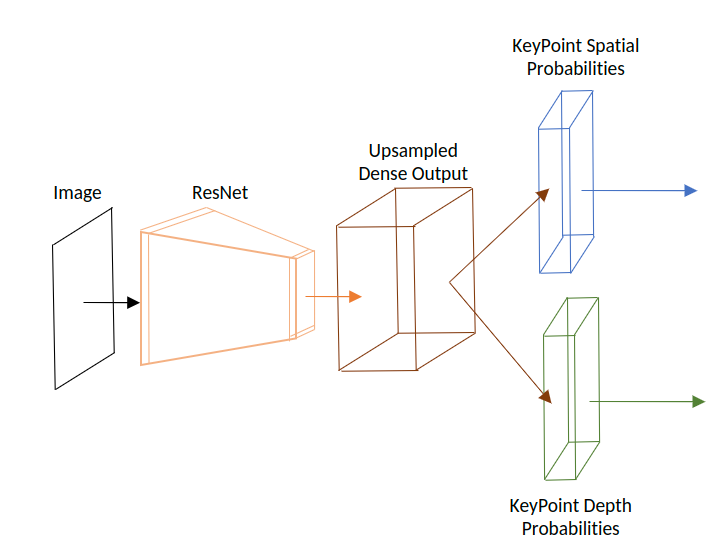
\includegraphics[scale=0.3]{images/keypointnet/arch.png}
\end{figure}